\chapter{Creazione del corpus e \textit{preprocessesing} dei dati}
Per analizzare al meglio le opinioni dei cittadini sul funzionamento dell'App Immuni si è scelto di soffermarci su ciò che essi scrivevano su Twitter, un social network molto popolare e utilizzato per esprimere in maniera semplice ed immediata opinioni riguardo ad una particolare tematica.

La scelta di utilizzare Twitter come strumento per la raccolta dei dati è giustificata anche da altri due fattori: innanzitutto, dal fatto che, rispetto ad altri social networks come Facebook e Instagram, Twitter è quello con la minore percentuale di profili privati, e in secondo luogo, dalla disponibilità di maggiori strumenti per la raccolta dei dati su questa piattaforma.

\section{La raccolta dei tweet utilizzando la libreria di \textit{scraping Twint}}
Si è scelto quindi di raccogliere i tweet scritti sul tema App Immuni durante un periodo temporale di un anno e mezzo, dal \textbf{1 giugno 2020}, mese in cui il Governo italiano ha rilasciato l'applicazione, fino alla fine dell'anno successivo (31 dicembre 2021). 
Per eseguire questa raccolta si è scelto di utilizzare una libreria di \textit{scraping} per la raccolta di tweet, la libreria \textit{Twint}\footnote{le cui informazioni sono reperibili all'interno del seguente repository GitHub: \url{https://github.com/twintproject/twint}}, una libreria Python ideata per  effettuare in maniera semplice e intuitiva lo scraping e con cui è possibile stabilire il termine di ricerca dei tweet (ad esempio gli hashtag, come nel nostro caso, o attraverso parole chiave) e il limite giornaliero di tweet da raccogliere, parametro utile soprattutto nel caso in cui si decida di raccogliere tweet in un range temporale più ampio o scritti su un fenomeno molto popolare e discusso.

Per poter raccogliere questi tweet sono stati utilizzati i tre principali hashtag scelti dagli utenti per discutere di questo fenomeno: \textit{Immuni}, \textit{ImmuniApp} e \textit{AppImmuni}.
Tramite l'utilizzo di questi hashtag sono stati raccolti i tweet pubblicati sia da utenti verificati, ossia appartenenti a celebrità o comunque persone riconosciute, identificate con la tipica spunta blu, che da utenti non verificati, così da avere un quadro più completo delle opinioni scritte anche da utenti comuni.

I seguenti tweet sono stati poi raccolti in base al giorno in cui sono stati scritti all'interno di file .json, con cui è stato poi possibile costruire due file .csv ciascuno contente i tweet raccolti con uno dei due hashtag, su cui avverrà poi l'intera analisi. 


\section{Comprensione dei dati}
Analizzando le caratteristiche interne dei dati raccolti si è notato come pur avendo lo stesso numero di colonne (36), quello creato utilizzando \#Immuni risulti più grande rispetto agli altri due: infatti mentre il primo conteneva circa 7mila righe, gli altri due contenevano rispettivamente 3789 e 2162 tweet.
Lo stesso fenomeno è visibile anche analizzando i valori delle singole colonne, in particolare il numero di \textbf{hashtag}, \textbf{tweet} e \textbf{utenti} (identificati univocamente con uno \textit{User Id}), come illustrato nella tabella
\ref{tab: info_ds}.

\begin{table}[H]
\centering
\begin{tabular}{|l|c|c|c|}
\hline
\rowcolor[HTML]{DAE8FC} 
\textbf{}                  & \textbf{\begin{tabular}[c]{@{}c@{}}Primo dataset \\ (\#Immuni)\end{tabular}} & \textbf{\begin{tabular}[c]{@{}c@{}}Secondo dataset \\ (\#AppImmuni)\end{tabular}} & \textbf{\begin{tabular}[c]{@{}c@{}}Terzo dataset  \\ (\#ImmuniApp)\end{tabular}} \\ \hline
\textit{Righe}             & 7032                                                                         & 3789                                                                              & 2162                                                                             \\ \hline
\textit{Colonne}           & 36                                                                           & 36                                                                                & 36                                                                               \\ \hline
\textit{Utenti (User\_id)} & 4706                                                                         & 978                                                                               & 1033                                                                             \\ \hline
\textit{tweet}            & 6885                                                                         & 1559                                                                              & 1602                                                                             \\ \hline
\textit{hashtag}          & 1068                                                                         & 833                                                                               & 796                                                                              \\ \hline
\end{tabular}
\caption{Confronto tra i valori dei due dataset e del dataset finale risultante dalla loro unione}
\label{tab: info_ds}
\end{table}
Dato che tutti i dataset contengono le stesse colonne, seppur con valori diversi, si è deciso di unirli così da avere un corpus più ampio per le analisi successive. Il dataset finale ha dunque le seguenti dimensioni: 12983 righe e 36 colonne. 

\section{Pulizia dei dati }
Infine, si è provveduto alla \textbf{pulizia} del dataset ottenuto, rimuovendo dapprima tutti i tweet duplicati, circa 3mila, ed eliminando tutte le colonne con valori nulli e quelle che, pur contenendo valori, non risultavano ottimali per le analisi successive, ad esempio la colonna \textit{translate}, \textit{conversation\_id}, \textit{created\_at}, \textit{time},	\textit{timezone},
come illustrato nella tabella \ref{tab:clean}.\\
Le dimensioni finali del dataset sono dunque le seguenti: 9784 righe e 11 colonne.\\


\begin{table}[H]
\centering
\begin{tabular}{|l|c|l|}
\hline
\multicolumn{1}{|c|}{\cellcolor[HTML]{DAE8FC}\textbf{\begin{tabular}[c]{@{}c@{}}Colonne Rimosse \\ (valori nulli)\end{tabular}}} & \multicolumn{1}{c|}{\cellcolor[HTML]{DAE8FC}\textbf{\begin{tabular}[c]{@{}c@{}}Colonne Rimosse \\ (inutili)\end{tabular}}} & \multicolumn{1}{c|}{\cellcolor[HTML]{DAE8FC}\textbf{Colonne mantenute}}         \\ \hline
place & quote\_url,  id    & date, username, name                    \\ \hline
thumbnail, near & created\_at, mention  & tweet, replies\_count                 \\ \hline
geo, surce retweet\_id & Conversation\_id & likes\_count, hashtag    \\ \hline
retweet\_date, translate  & urls, photos, timezone  & retweet\_count, user\_id                    \\ \hline
trans\_src , trans\_dest  & video, cashtags & reply\_to, name                   \\ \hline
\end{tabular}
\caption{Valori eliminati dal corpus durante la fase di pulizia}
\label{tab:clean}
\end{table}


\section{Analisi dei tweet più popolari e il loro andamento temporale}
Dopo aver creato e pulito il dataset finale, si è continuato ad analizzare alcuni aspetti che potessero fornire ulteriori informazioni utili per l'analisi.

Innanzitutto, si è scelto di analizzare i \textbf{tweet più popolari}, ordinandoli in base al numero di \textit{retweet} (ossia di volte in cui gli utenti hanno condiviso il tweet sul proprio profilo), di \textit{likes} (cioè quante volta gli utenti hanno espresso il loro gradimento cliccato sul simbolo 'mi piace' corrispondente al cuoricino posto in basso a sinistra di ciascun tweet)  e di menzioni (cioè il numero di risposte che gli utenti hanno lasciato sotto quel tweet).

Da questa analisi sono emersi alcuni aspetti, come il fatto che molto spesso i tweet più virali siano quelli scritti da personaggi molto influenti, soprattutto figure politiche, i quali esprimono non tanto la loro non fiducia nella applicazione quanto il loro disappunto nei riguardi del lavoro svolto cariche istituzionali, come mostra il tweet scritto dall'Onorevole Daniela Santanché, la quale il 10 ottobre 2020 scrive che non ha intenzione di cedere i propri dati sensibili ad un applicazione per cui il Governo non ha fornito linee guida chiare.\\
Il suddetto tweet è in assoluto quello con più risposte (334 risposte totali), in cui gli utenti esprimono sia il loro accordo con l'affermazione dell'Onorevole sia il fatto che i dati che l'utente fornisce all'applicazione sono gli stessi che inconsapevolmente cede anche ad altre piattaforme social o a siti web in generale.\\
Questo fenomeno secondo cui le persone più influenti sono quelle con cui gli utenti interagiscono maggiormente può essere confermato dal fatto che Twitter e in generale tutti i social networks possono essere visti come una grande rete sociale formata dalle interazioni tra gli utenti, che nel caso di Twitter sono rappresentati dai likes, commenti, retweet e risposte che gli utenti lasciano sotto ai vari tweet. All'interno della rete esistono poi dei nodi (in questo caso utenti) più influenti di altri che solitamente corrispondono alle persone più influenti nella società (celebrità, figure politiche e religiose ecc.), i quali sono collegati a più persone e hanno quindi maggiori probabilità di interagire maggiormente con gli utenti.

%Queste persone sono solitamente celebrità, figure religiose e figure politiche, come nel caso della nostra analisi in cui spesso i tweet con più interazione in assoluto sono quelli scritti da figure politiche,  % inserire commento sull'influenza di alcuni nodi con degree centrality più ampia, inserendo anche il fatto che in realtà twitter e in generale i social possono essere visti come una rete formata da nodi (utenti) e relazioni (commenti, likes, rt e in generale le interazioni ai tweet)

Analizzando altri tweet molto popolari emergono spesso toni ironici nei confronti dell'applicazione e dei pochi download ricevuti. Addirittura, in uno dei tweet con più retweet e likes, un utente afferma come addirittura i download di un’applicazione come la torcia del cellulare superino quelli dell'app Immuni, nascondendo sotto questa affermazione ironica un dato di fatto: gli utenti non scaricano l'applicazione.
Un altro aspetto interessante che si è scelto di analizzare è l’andamento temporale dei tweet per cercare di individuare eventuali periodi in cui la discussione su Immuni era particolarmente accesa cercando poi un riscontro su ciò che stava avvenendo in quel periodo e individuando quindi se ci fosse un evento che avesse influito sulla discussione.
\begin{figure} [H]
    \centering
    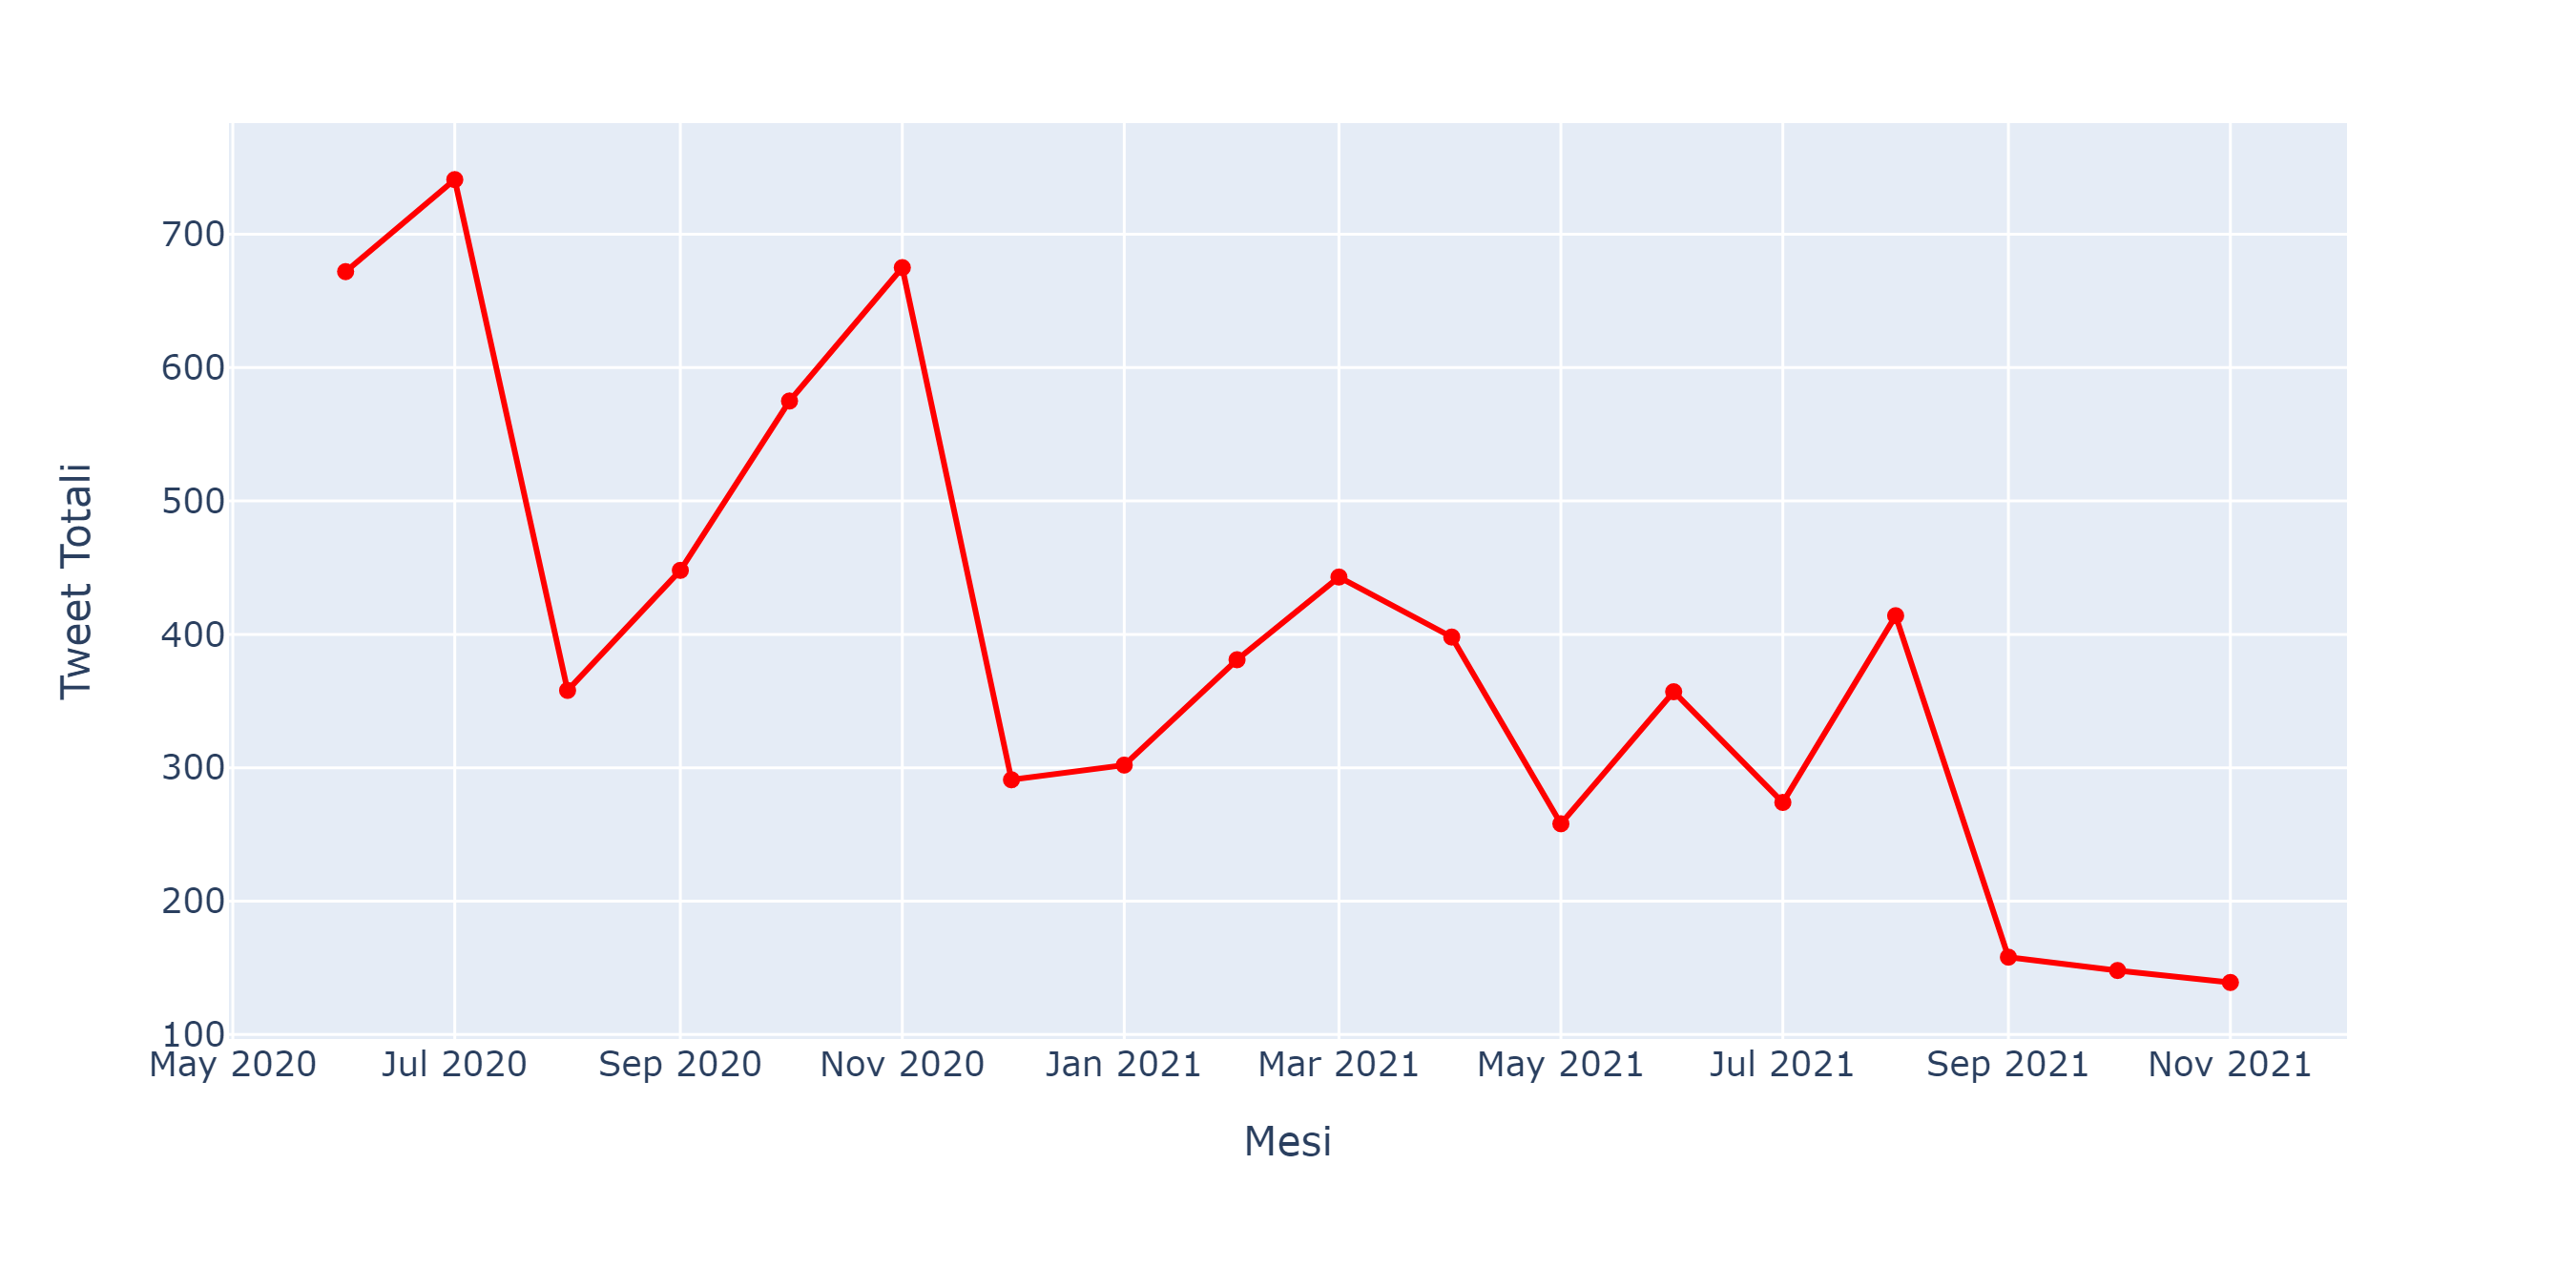
\includegraphics[width = 1\textwidth]{img/tweet_mesi.png}
    \caption{Andamento temporale dei tweet pubblicati sull'app Immuni tra giugno 2020 e dicembre 2021}
    \label{fig:tweet_mesi}
\end{figure}
Come si può vedere dal grafico in figura \ref{fig:tweet_mesi} ci sono stati alcuni periodi in cui c'è stato un maggiore dibattito tra gli utenti sul tema app Immuni, come quello avvenuto tra giugno e luglio 2020, mesi in cui per la prima volta l'applicazione viene rilasciata a livello nazionale su tutti gli store digitali e in cui sono stati scritti in totale 1414 tweet (672 a giugno e 741 a luglio), per poi riprendere a ottobre e novembre 2020, mesi in cui i contagi sono aumentati esponenzialmente dopo il calo durante i mesi estivi, con circa 600mila casi al giorno\footnote{Fonte: Monitoraggio situazione Covid-19 della Protezione Civile, disponibile all'indirizzo: \url{https://mappe.protezionecivile.gov.it/it/mappe-emergenze/mappe-coronavirus/situazione-desktop}}, fenomeno che ha portato gli utenti a discutere nuovamente sul tema e sulla sua efficacia nel monitoraggio dei casi. %Inoltre, in quel periodo, sono state stanziate le cosiddette "zone", dove in base al numero di contagi registrati in una regione ad essa veniva assegnato un colore (rosso, giallo, bianco) che rappresentavano un maggiore numero di restrizioni per la popolazione in termini di spostamenti dentro e fuori dalla regione e accesso ai luoghi pubblici.  % da rivedere
In questi mesi il totale dei tweet scritti sul tema è leggermente inferiore a quelli scritti a giugno e luglio (1250 tweet in totale).

A partire dal 2021, invece, la discussione sull'app Immuni comincia a diminuire con una media di 300 tweet al mese, per poi calare nei mesi finali, con un media di circa 150 tweet scritti nei mesi di settembre, ottobre e novembre 2021, un numero molto inferiore rispetto a quelli dell'anno precedente. Questo dato è probabilmente dovuto alla scarsa promozione dell'applicazione da parte delle cariche istituzionali, ma anche dalla riduzione delle misure restrittive grazie all'inizio della campagna vaccinale.

Tuttavia, ad agosto 2021 si registra un leggero aumento dei tweet sul tema (414 tweet), forse dovuto all'introduzione come stabilito dal Decreto Legge n 105 del 23/07/2021\footnote{D.L. n 105 23/07/2021, consultabile sulla Gazzetta Ufficiale all'indirizzo: \url{https://www.gazzettaufficiale.it/eli/id/2021/07/23/21G00117/sg})} della Certificazione Verde o \textit{Green Pass}, uno strumento scaricabile sul sito del Governo, che veniva assegnato ai cittadini guariti da Covid o che avevano ricevuto una o due dosi di vaccino che permette di accedere a molti servizi pubblici come scuole, luoghi di intrattenimento e strutture sanitarie. 
Questo fenomeno è in qualche modo collegato all'app Immuni, in quanto in quel periodo all'interno dell'applicazione è stata implementata la funzione di poter contenere il Green Pass in modo tale da facilitarne la reperibilità da parte dei cittadini. 
Tuttavia, questa nuova funzione sembra non aver risolto i problemi e lo scarso successo dell'applicazione che infatti nei mesi successivi è tornata ad essere inutilizzata.








